\documentclass[aspectratio=43]{beamer}
% Theme works only with a 4:3 aspect ratio
\usetheme{CSCS}

\usepackage{tikz}
\usepackage{pgfplots}
\usepackage{pgfplotstable}
\usetikzlibrary{pgfplots.groupplots,spy,patterns}
\usepackage{listings}
\usepackage{color}
\usepackage{tcolorbox}
\usepackage{anyfontsize}
\usepackage{xspace}
\usepackage{graphicx}

% define footer text
\newcommand{\footlinetext}{Introduction to GPUs in HPC}

% Select the image for the title page
\newcommand{\picturetitle}{cscs_images/image5.pdf}

% fonts for maths
\usefonttheme{professionalfonts}
\usefonttheme{serif}

% source code listing
\newcommand{\axpy}{{\ttfamily axpy}\xspace}

% set indent to a more reasonable level (so that itemize can be used in columns)
\setlength{\leftmargini}{20pt}

\DeclareTextFontCommand{\emph}{\bfseries\color{blue!70!black}}

% Please use the predifined colors:
% cscsred, cscsgrey, cscsgreen, cscsblue, cscsbrown, cscspurple, cscsyellow, cscsblack, cscswhite

\author{Ben Cumming, CSCS}
\title{Writing GPU Kernels}
\subtitle{}
\date{\today}

\begin{document}

% TITLE SLIDE
\cscstitle

% CHAPTER SLIDE
\cscschapter{Going Parallel : Kernels and Threads}

%%%%%%%%%%%%%%%%%%%%%%%%%%%%%%%%%%%%%%%%%%%%
\begin{frame}[fragile]{Threads and Kernels}
%%%%%%%%%%%%%%%%%%%%%%%%%%%%%%%%%%%%%%%%%%%%
    \begin{itemize}
        \item \emph{Threads} are streams of execution, run simultaneously on GPU.
        \item A \emph{kernel} is the function run by each thread.
        \item CUDA provides language support for:
        \begin{itemize}
            \item writing kernels;
            \item launching many threads to execute a kernel in parallel.
        \end{itemize}
        \item CUDA hides the low-level details of launching threads.
    \end{itemize}

    \begin{info}{The process for developing CUDA kernels}
        \begin{enumerate}
            \item Formulate algorithm in terms of parallel work items.
            \item Write a kernel implementing a work item on one thread.
            \item Launch the kernel with the required number of threads.
        \end{enumerate}
    \end{info}
\end{frame}

%%%%%%%%%%%%%%%%%%%%%%%%%%%%%%%%%%%%%%%%%%%%
\begin{frame}[fragile]{Scaled Vector Addition (\axpy)}
%%%%%%%%%%%%%%%%%%%%%%%%%%%%%%%%%%%%%%%%%%%%
    We have used CUBLAS to perform scaled vector addition:
        $$\mathbf{y} = \mathbf{y} + \alpha \mathbf{x}$$
        \vspace{-15pt}
    \begin{itemize}
        \item $\mathbf{x}$ and $\mathbf{y}$ are vectors of length $n$; \hfill $x,y \in \mathbb{R}^n$
        \item $\alpha$ is scalar. \hfill $\alpha\in\mathbb{R}$
    \end{itemize}
    Applying \axpy requires $n$ operations:
    $$y_i \leftarrow y_i + a*x_i,\quad i = {0, 1, \dots, n-1}$$
    which can be performed \emph{independently} and \emph{in any order}.

    \begin{code}{\axpy implemented on CPU with a loop}
%..................................
        \begin{lstlisting}[style=boxcuda]
void axpy(double *y, const double *x, double a, int n) {
  for(int i=0; i<n; ++i)
    y[i] = y[i] + a*x[i];
}
        \end{lstlisting}
%..................................
    \end{code}

\end{frame}

%%%%%%%%%%%%%%%%%%%%%%%%%%%%%%%%%%%%%%%%%%%%
\begin{frame}[fragile]{Kernels}
%%%%%%%%%%%%%%%%%%%%%%%%%%%%%%%%%%%%%%%%%%%%
    A \emph{kernel} defines the work item for a single thread
    \begin{itemize}
        \item The work is performed by many threads executing the same kernel \emph{simultaneously}.
        \item Conceptually corresponds to the inner part of a loop for BLAS1 operations like \axpy.
    \end{itemize}

    \vspace{-10pt}
    \begin{columns}[T]
        \begin{column}{0.5\textwidth}
            \begin{codecolumn}{host : add two vectors}
%..................................
        \begin{lstlisting}[style=boxcudatiny]

void add_cpu(int *a, int *b, int n){
  for(auto i=0; i<n; ++i)
    a[i] = a[i] + b[i];
}
        \end{lstlisting}
%..................................
            \end{codecolumn}
        \end{column}
        \begin{column}{0.5\textwidth}
            \begin{codecolumn}{CUDA : add two vectors}
%..................................
        \begin{lstlisting}[style=boxcudatiny]
__global__
void add_gpu(int *a, int *b, int n){
  auto i = threadIdx.x;
  a[i] = a[i] + b[i];
}
        \end{lstlisting}
%..................................
            \end{codecolumn}
        \end{column}
    \end{columns}

    \vspace{-2pt}
    \begin{info}{}
    \begin{itemize}
        \item \lst{__global__} keyword indicates a kernel
        \item \lst{threadIdx} used to find unique id of each thread
    \end{itemize}
    \end{info}
\end{frame}

%%%%%%%%%%%%%%%%%%%%%%%%%%%%%%%%%%%%%%%%%%%%
\begin{frame}[fragile]{Launching a kernel}
%%%%%%%%%%%%%%%%%%%%%%%%%%%%%%%%%%%%%%%%%%%%
    \begin{itemize}
        \item Host code launches a kernel on the GPU \emph{asynchronously}.
        \item CUDA provides the ``triple chevron'' \lst{``<<<``_,_``>>>``} syntax for launching a kernel.
    \end{itemize}

    \begin{columns}[T]
        \begin{column}{0.5\textwidth}
            \begin{codecolumn}{host : add two vectors}
%..................................
        \begin{lstlisting}[style=boxcuda]
auto n = 1024;
auto a = host_malloc<int>(n);
auto b = host_malloc<int>(n);
add_cpu(a, b, n);
        \end{lstlisting}
%..................................
            \end{codecolumn}
        \end{column} \begin{column}{0.5\textwidth}
            \begin{codecolumn}{CUDA : add two vectors}
%..................................
        \begin{lstlisting}[style=boxcuda]
auto n = 1024;
auto a = device_malloc<int>(n);
auto b = device_malloc<int>(n);
add_gpu@<<<@1,n@>>>@(a, b, n);
        \end{lstlisting}
%..................................
            \end{codecolumn}
        \end{column}
    \end{columns}

    \begin{itemize}
        \item \lst{add_gpu``<<<``1, num_threads``>>>``(args... )} launches the kernel \lst{add_gpu} with \lst{num_threads} parallel threads.
    \end{itemize}

\end{frame}

%%%%%%%%%%%%%%%%%%%%%%%%%%%%%%%%%%%%%%%%%%%%
\begin{frame}[fragile]{Exercise: My First Kernel}
%%%%%%%%%%%%%%%%%%%%%%%%%%%%%%%%%%%%%%%%%%%%
    Open \lst{axpy/axpy.cu}

    \begin{enumerate}
        \item Write a kernel that implements \axpy for \lst{double}
        \begin{itemize}
            \item \lst{axpy_kernel(double *y, double *x, double a, int n)}
            \item \extra can you write a C++ templated version for any type?
        \end{itemize}

    \item launch the kernel (look for \lst{TODO})
        \item Compile the test and run
        \begin{itemize}
            \item it will pass with no errors on success
            \item first try with small vectors of size 8
            \item try increasing launch size... what happens?
        \end{itemize}
        \item \extra can you extend the kernel to work for larger arrays?
    \end{enumerate}
\end{frame}



% CHAPTER SLIDE
\cscschapter{Scaling Up : Thread Blocks}

%%%%%%%%%%%%%%%%%%%%%%%%%%%%%%%%%%%%%%%%%%%%
\begin{frame}[fragile]{}
%%%%%%%%%%%%%%%%%%%%%%%%%%%%%%%%%%%%%%%%%%%%
    \begin{info}{}
        In the \axpy exercises we were limited to 1024 threads for a kernel launch
        \begin{itemize}
            \item but we need to scale beyond 1024 threads for the \emph{massive parallelism} we were promised!
        \end{itemize}
    \end{info}

    \begin{info}{Thread blocks and grids}
        kernels are executed in groups of threads called \emph{thread blocks}
        \vspace{-12pt}
        \begin{itemize}
            \item the launch configuration \lst{axpy``<<<``grid_dim, block_dim``>>>``(...)}
            \begin{itemize}
                \item launch a \emph{grid} of \lst{grid_dim} \emph{blocks}
                \item each \emph{block} has \lst{block_dim} \emph{threads}
                \item for a total of \lst{grid_dim}$\times$\lst{block_dim} threads
            \end{itemize}
            \item previously we launched just one thread block \lst{axpy``<<<``1, n``>>>``(...)}
        \end{itemize}
    \end{info}

\end{frame}

%%%%%%%%%%%%%%%%%%%%%%%%%%%%%%%%%%%%%%%%%%%%
\begin{frame}[fragile]{Why the additional complexity?}
%%%%%%%%%%%%%%%%%%%%%%%%%%%%%%%%%%%%%%%%%%%%
        \emph{Coordination between threads doesn't scale:}
        \begin{itemize}
            \item Threads in a block can synchronize and share resources
            \item This does not scale past a certain number of cores/threads
            \item EACH P100 GPU \emph{streaming multiprocessor} (SMX) has 64 CUDA cores, and can run 2048 threads
            \item Threads in a block run on the same SMX, with shared resources and thread cooperation
            \item Work is broken into blocks, which are distributed over the 56 SMXs on the GPU.
        \end{itemize}
\end{frame}

%%%%%%%%%%%%%%%%%%%%%%%%%%%%%%%%%%%%%%%%%%%%
\begin{frame}[fragile]{}
%%%%%%%%%%%%%%%%%%%%%%%%%%%%%%%%%%%%%%%%%%%%
\begin{center}
\vspace{-0.75cm}
\begin{tabular}{|c|m{4cm}|m{5cm}|}
    \cline{1-2}
        concept & hardware &  \multicolumn{1}{c}{} \\
    \hline
        thread &
        \begin{minipage}{4cm}
            \includegraphics[width=0.3\textwidth]{./images/core.pdf}
        \end{minipage} &
        \footnotesize
        \begin{itemize}
            \item each thread executed on one core
        \end{itemize} \\
    \hline
        block &
        \begin{minipage}{4cm}
            \includegraphics[width=0.3\textwidth]{./images/smx.pdf}
        \end{minipage} &
        \footnotesize
        \begin{itemize}
            \item block executed on 1 SMX
            \item multiple blocks per SMX if sufficient resources
            \item threads in a block share SMX resources
        \end{itemize} \\
    \hline
        grid &
        \begin{minipage}{4cm}
            \includegraphics[width=0.3\textwidth]{./images/smx.pdf}
            \includegraphics[width=0.3\textwidth]{./images/smx.pdf}
            \includegraphics[width=0.3\textwidth]{./images/smx.pdf}
        \end{minipage} &
        \footnotesize
        \begin{itemize}
            \item kernel is executed in grid of blocks
            \item blocks distributed over SMXs
            \item multiple kernels can run at same time
        \end{itemize} \\
\hline
\end{tabular}
\end{center}
\end{frame}

%%%%%%%%%%%%%%%%%%%%%%%%%%%%%%%%%%%%%%%%%%%%
\begin{frame}[fragile]{Calculating thread indexes}
%%%%%%%%%%%%%%%%%%%%%%%%%%%%%%%%%%%%%%%%%%%%
        A kernel has to calculate the index of its work item
        \begin{itemize}
            \item In \lst{axpy} we used \lst{threadIdx.x} for the index.
            \item With multiple blocks, we need more information, which is available in the following \emph{magic variables}:
        \end{itemize}

    \begin{info}{}
        \begin{center}
            \begin{tabular}{ll}
            \lst{gridDim}   &: total number of blocks in the grid \\
            \lst{blockDim}  &: number of threads in a thread block \\
            \lst{blockIdx}  &: index of block \lst{[0, gridDim-1]} \\
            \lst{threadIdx} &: index of thread in thread block \lst{[0, blockDim-1]} \\
            \end{tabular}
        \end{center}
    \end{info}

\end{frame}

%%%%%%%%%%%%%%%%%%%%%%%%%%%%%%%%%%%%%%%%%%%%
\begin{frame}[fragile]{Calculating thread indexes}
%%%%%%%%%%%%%%%%%%%%%%%%%%%%%%%%%%%%%%%%%%%%
        Consider accessing an array of length 24 with 8 threads per block. The \emph{dimensions} of the kernel launch are:
        \begin{itemize}
            \item \lst{blockDim.x == 8} (8 threads/block)
            \item \lst{gridDim.x == 3} (3 blocks)
        \end{itemize}
        We calculate the index for our thread using the formula
        \begin{center}
            \lst{auto index = threadIdx.x + blockIdx.x*blockDim.x}\\
            \vspace{0.5cm}
            \centering 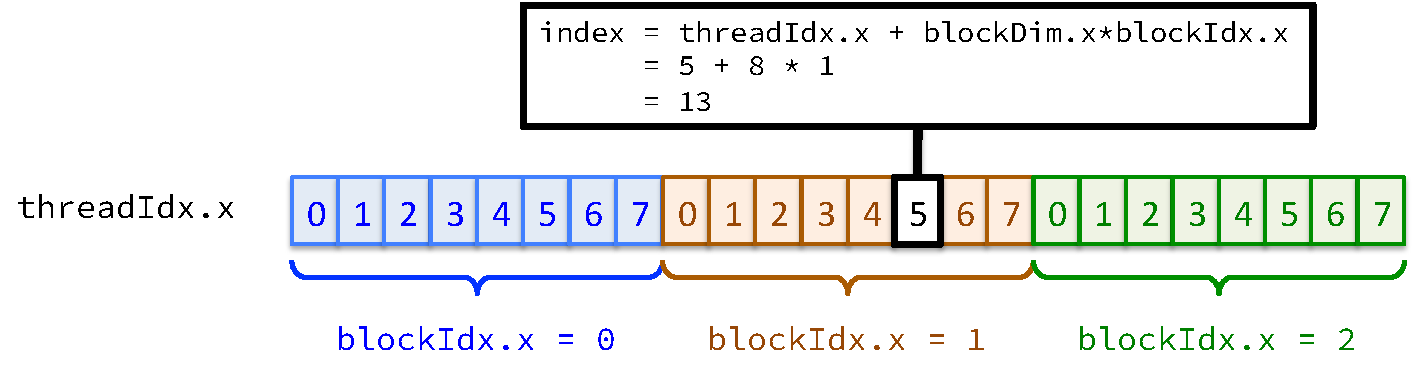
\includegraphics[width=\textwidth]{./images/blocks.pdf}
        \end{center}
\end{frame}

%%%%%%%%%%%%%%%%%%%%%%%%%%%%%%%%%%%%%%%%%%%%
\begin{frame}[fragile]{Calculating grid dimensions}
%%%%%%%%%%%%%%%%%%%%%%%%%%%%%%%%%%%%%%%%%%%%
            The number of thread blocks and the number of threads per block are parameters for the kernel launch:
            \begin{center}
                \lst{kernel``<<<``blocks, threads_per_block``>>>``(...)}
            \end{center}
            Remember to guard against overflow when the number of work items is not divisible by the thread block size

    \begin{code}{vector addition with multiple blocks}
%..................................
        \begin{lstlisting}[style=boxcudatiny]
__global__
void add_gpu(int *a, int *b, int n){
  auto i = threadIdx.x + blockIdx.x*blockDim.x;
  if(i<n) { // guard against access off end of arrays
    a[i] += b[i];
  }
}

// in main()
auto block_size = 512;
auto num_blocks = (n + (block_size-1)) / block_size;
add_gpu@<<<@num_blocks, block_size@>>>@(a, b, n);
        \end{lstlisting}
%..................................
    \end{code}
\end{frame}

%%%%%%%%%%%%%%%%%%%%%%%%%%%%%%%%%%%%%%%%%%%%
\begin{frame}[fragile]{Calculating grid dimensions}
%%%%%%%%%%%%%%%%%%%%%%%%%%%%%%%%%%%%%%%%%%%%
        We have to take care when calculating the number of blocks in the grid, i.e. \lst{blocks}:
        \begin{center}
            \lst{kernel``<<<``blocks, threads_per_block``>>>``(...)}
        \end{center}
        Most likely, the number of work items \lst{n} is not a multiple of \lst{threads_per_block}
        \begin{itemize}
            \item some threads in the last thread block will be idle.
        \end{itemize}

    \begin{code}{Calculating grid dimensions}
%..................................
        \begin{lstlisting}[style=boxcudatiny]
// in main()
auto block_size = 512;
auto num_blocks = (n + block_size-1) / block_size;
add_gpu@<<<@num_blocks, block_size@>>>@(a, b, n);
        \end{lstlisting}
%..................................
    \end{code}
\end{frame}

%%%%%%%%%%%%%%%%%%%%%%%%%%%%%%%%%%%%%%%%%%%%
\begin{frame}[fragile]{How many threads per block?}
%%%%%%%%%%%%%%%%%%%%%%%%%%%%%%%%%%%%%%%%%%%%
    The number of threads per block has an impact on performance
    \begin{itemize}
        \item The optimal number depends on resources required by the kernel (registers, shared memory, computational intensity, etc).
    \end{itemize}
    The short answer is 64 or 128 on P100.
    \begin{itemize}
        \item For the main kernels in your application, perform experiments to find the ideal block size.
    \end{itemize}
\end{frame}

%%%%%%%%%%%%%%%%%%%%%%%%%%%%%%%%%%%%%%%%%%%%
\begin{frame}[fragile]{Exercise: Blocks}
%%%%%%%%%%%%%%%%%%%%%%%%%%%%%%%%%%%%%%%%%%%%
    Open \lst{axpy/axpy.cu} from the last exercise
    \begin{enumerate}
        \item Extend the \axpy kernel for arbitrarily large input arrays (any \lst{n})

        \item Update the call site to calculate the grid configuration

        \item Compile the test and run
        \begin{itemize}
            \item it will pass with no errors on success
        \end{itemize}

        \item Experiment with varying the size of the arrays (scaling)
        \begin{itemize}
            \item start small and increase
        \end{itemize}

        \item finish the \lst{newton.cu} example
        \begin{itemize}
            \item how do the h2d, d2h and kernel timings compare?
        \end{itemize}

        \item \extra Compare scaling with the \lst{axpy_omp} benchmark

        \item \extra Experiment with varying the block size

    \end{enumerate}

\end{frame}

%%%%%%%%%%%%%%%%%%%%%%%%%%%%%%%%%%%%%%%%%%%%
\begin{frame}[fragile]{Exercise: Results}
%%%%%%%%%%%%%%%%%%%%%%%%%%%%%%%%%%%%%%%%%%%%

\begin{center}
\begin{tikzpicture}
    \pgfplotsset{footnotesize}
    \begin{axis}[
        height=0.4\textwidth,
        width=\textwidth,
        xmin=10,xmax=29,
        ymin=0,ymax=8,
        xtick={10,12,14,16,18,20,22,24,26,28},
        ytick={0,1,2,3,4,5,6,7,8},
        xlabel=$log_2(n)$,
        ylabel=speedup,
        legend style = {at={(0.05,0.95)}, anchor=north west},
        every axis y label/.style=
            {at={(ticklabel cs:0.5)},rotate=90,anchor=near ticklabel},
        grid=major]
        \addplot[color=blue,mark=*]  table[x=n,y expr=\thisrow{openmp}/\thisrow{cuda}]  {./plots/omp_axpy.tbl};
        \addplot[color=black,mark=*] table[x=n,y expr=\thisrow{openmp}/\thisrow{openmp}] {./plots/omp_axpy.tbl};
        \legend{CUDA speedup, OpenMP};
    \end{axis}
\end{tikzpicture}
\end{center}

The GPU is a throughput device:
\begin{itemize}
\item CUDA breaks even for $n \geq 2^{14}\approx 16,000$
\item requires $2^{21}\approx2,000,000$ to gain ``full'' $7\times$ speedup
\end{itemize}
You have to provide enough parallelism to exploit many cores

\end{frame}

\end{document}

